\section*{Rough Draft}
This dissimilarity leads to time-inconsistency problems, where in the short-term countries prefer either less severe economic or political conditions instead of minimizing the joint conditionality over the long-term.


One implication is that more democratic countries should be more sensitive to explicitly political conditions and, thus, prefer Western loans $ceteris\;paribus$. 

\subsubsection*{Figure 1: Non-Democratic Country Loan Preference, $ceteris\;paribus$}
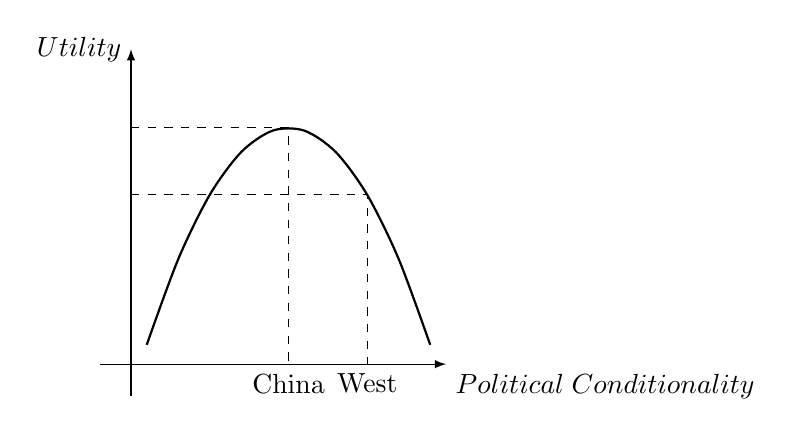
\begin{tikzpicture}[scale=2,declare function={F(\x) = 1.7*(2*\x-\x*\x)-0.2;}]
  \draw[-latex] (0,-0.2) -- (0,2) node[left]{$Utility$};
  \draw[-latex] (-0.2,0) -- (2,0) node[below right]{$Political\;Conditionality$};
  \draw[domain=0.1:1.9,samples=10,smooth,thick] plot (\x, {F(\x)}); 
  \coordinate (max) at (0,{F(1)});
  \draw[dashed] (max) -| (1,0) node[pos=1,below]{China};
  \coordinate (max) at (0,{F(1.5)});
  \draw[dashed] (max) -| (1.5,0) node[pos=1,below]{West};
\end{tikzpicture}

\section*{Idea Brief}
\subsection*{What needs to be explained}
Given the seeming consensus of economic and political deglobalization,  namely in the West, there is attention being paid to China's position in this story, whether as a cause or of an effect. Regardless, I argue that China's eminence in the foreign aid spending increases donor competition for foreign aid and leads to a reduction in perceived concessions on behalf of the recipient. Further, autocratic countries are likely to disproportionately benefit from this concession deficit and thus work more with China more than democracies. Can I formalize this?

Differences between money flows: aid (grants) versus loans (debt) and official da (ODA) and (OOF) (ODA like flows less economically self-interested, Dreher?)
------

Developing countries seem to have an increased ability to choose donors for foreign aid. Not only has China been giving an incredible amount of aid, but now the U.S. and G7 are expanding their aid opportunities. Given this phenomenon, how do aid-seeking countries decide between bilateral donors and international institutions like the IMF and World Bank? And, how does choosing Chinese money over IMF funds, for instance, affect the politics of the recipient country? In other words, what is the political difference between receiving money from international organizations and other entities, like the U.S. or China? Is the BRI really an attractive substitute for IMF funding?

----------
Supply side focus thus far (how donor behavior has been affected).
Lots of academic attention on supply side provision of aid given China's entrance (e.g., \scite{dreher2018}, \cite{dreher2015}), but few explorations of the demand side after China has become a prevalent donor. Also research on how Chinese aid affects recipients in various ways (e.g., \cite{martorano2020}, \cite{bader2015}).
This paper seeks to address this shortage in the literature, aiming to understand how recipient countries choose between the vast number of credible donors. Relevant literature: \cite{kilama2016a}, \cite{hernandez2017}, \cite{li2017a}, \cite{isaksson2018}, \cite{humphrey2019}, \cite{broich2017a}.

\subsection*{Theory} 
Given that there are more than one donors offering money, recipients pick the sum that maximizes their utility. Their utility function has two parameters: net value of the sum minus the cost of concessions to the donor. Assumption: 1) donors have strategic interests that define who they give money to 2) democratic countries and international institutions have weakly democratic strategic aims whereas autocratic donors have weakly autocratic aims. 

One period game. Competition when more than one donor present, where recipient can choosing between IMF loan and investment from other countries. Countries compete by offering more money or lowering concessions required. What about reneging? (recipients less likely to renege when donor matches their policy preference as concessions are lower? Or reputation loss and inability to get future monies?)  Implications being that countries have had to make less concessions over time due to competition and tend to accept money from donors with similar preferences, if available.

\textbf{Expected Implications} 
\begin{align*}
    H_1:\; &\text{Autocratic recipients choose to rather receive money from autocratic donors than}\\
    &\text{international organizations or democratic donors.}\\
    H_2:\; &\text{Recipients of (democratic) autocratic aid will become weakly more (democratic) autocratic.}
\end{align*}

\subsection*{Alternative Explanations}

\subsection*{Methodology}
Some descriptive stats on foreign aid spending by country and organization over time. 

Test: Look at countries who previously received IMF funding who switched to Chinese money, use it as treatment?

\subsection*{Complications}
